\documentclass[a4paper, 12pt,]{scrartcl}



\usepackage[utf8]{inputenc}

\usepackage[ngerman]{babel}
\usepackage{amssymb}
\usepackage[T1]{fontenc}
\usepackage{mathtools}
\usepackage{amsmath}
\usepackage{ntheorem}
\usepackage{bbm}
\usepackage{dsfont}
\usepackage{color}
\usepackage{slashed}
\usepackage{hyperref}
\usepackage{graphicx} 
\usepackage{bm}
\usepackage{mathabx}
\usepackage{float}
\usepackage{mwe}
\usepackage{multirow}
\begin{document}
\begin{titlepage}
	\centering
	{\scshape\LARGE Universität Tübingen \par}
	\vspace{2cm}
	{\huge\bfseries Sterling Motor \par}
	\vspace{2cm}
	{\Large \scshape Blockpraktikum 2021} \par
	\vspace{2cm}
	{\Large  Erste Version} \par
	\vspace{2cm}
	{\Large\itshape \underline{Christian Gommeringer} \space \space  \underline{Matthias Gatter}\par}
	\vfill 
	{\large betreut von Jan Riedelsheimer}
	\vfill

	{\large \today\par}
\end{titlepage}
\newpage 
\tableofcontents 

\newpage
\section{Einleitung}
\begin{flushleft}

In diesem Versuch betrachten wir einen realen Stirling Motor und wollen dessen Funktionsweise thermodynamisch verstehen und seine wichtigsten Parameter experimentell bestimmen.

\end{flushleft}
% > < | 
\section{Theorie}
Unseren Überlegungen zugrunde liegt der Sterling Kreisprozess
\begin{figure}[H]\centering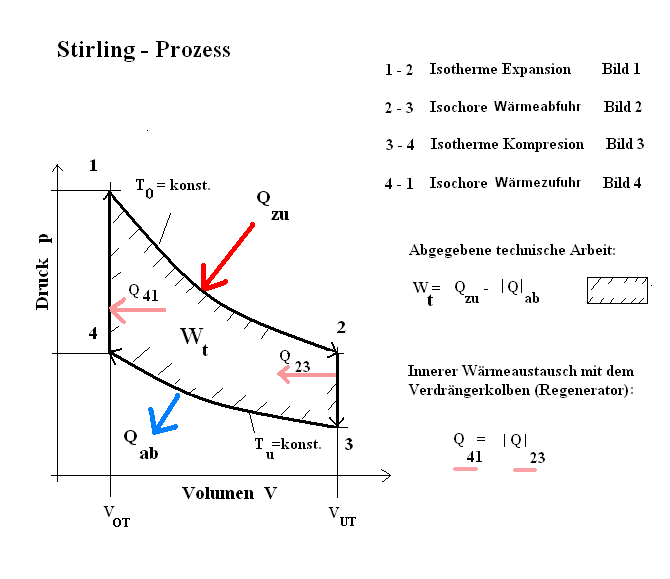
\includegraphics[scale=0.5]{Stirling-Prozess_3}\caption{Abbildung des stirlingschen Kreisprozesses aus Wikipedia}\end{figure}
Wenn wir ihn in der oben abgebildeten Reihenfolge durchlaufen, lässt sich die Wärme, die vom Arbeitsgas mit den Wärmebädern ausgetauscht wurde, in folgende Abschnitte aufteilen
\begin{gather*}\Delta{Q}_{12}=\text{ln}\left(\frac{V_2}{V_1}\right)\,n\,R\,T_1\\
\Delta{Q}_{23}=C_v\,(T_3-T_1)\\
\Delta{Q_{34}}=-\text{ln}\left(\frac{V_2}{V_1}\right)\,n\,R\,T_3\\
\Delta{Q_{41}}=C_v\,(T_1-T_3)\end{gather*}
Hierbei ist $T_1>T_3$. Dies wollen wir in den gesamten folgenden Überlegungen beibehalten. Betrachten wir nun die Energieaustauschbilanz der Wärmebäder, erhalten wir diese indem wir den Energieaustauschs des Arbeitsgases negieren. Damit lässt sich die Bilanz $\Delta{Q_{B_1}}$ für das wärmere Bad mit Temperatur $T_1$ und für das kältere Bad $\Delta{Q_{B_2}}$ aufstellen.
\begin{gather*}\Delta{Q_{B_1}}=-\Delta{Q}_{12}-\Delta{Q_{41}}=-\text{ln}\left(\frac{V_2}{V_1}\right)\,n\,R\,T_1-C_v\,(T_1-T_3)\\
\Delta{Q_{B_2}}=-\Delta{Q}_{34}-\Delta{Q_{23}}=\text{ln}\left(\frac{V_2}{V_1}\right)\,n\,R\,T_3+C_v\,(T_1-T_3)\end{gather*}
Die Beschreibung bezog sich jetzt zuerst auf die Bilanzen beim Betrieb als Wärme-Kraft-Maschine. Der gleiche Wärmetransport wird auch geleistet wenn das System durch einen externen Motor in dieser Richtung betrieben wird (im folgenden wird dieser Umlaufsinn als Umlaufsinn1 bezeichnet). Hier wird Wärmebad 1 gekühlt und Wärmebad 2 beheizt. Der Vorteil des Betriebs durch den Motor, ist dass sich so durch mehr Umdrehungen pro Minute eine stärkere Kühlleistung erbringen lässt oder überhaupt eine Kühlleistung, falls der Temperatur zu gering ist um die Wärmekraftmaschine überhaupt in Gang zu bringen. Die Kühlwirkung bezieht sich auf das Wärmebad 1, das in unserem Fall der Zylinderkopf ist. \newline
Durch Umkehren des Durchlaufs des Stirling Prozesses lässt sich der Zylinderkopf auch heizen. Hier ist allerdings zu beachten, dass von $1\rightarrow4$ das kältere Wärmebad Wärme aufnimmt und von $3\rightarrow2$ das Wärmebad 1 Wärme abgibt. Die Bilanz für die Wärmebäder ergibt sich daher als
\begin{gather*}\Delta{Q_{B_1}}'=\text{ln}\left(\frac{V_2}{V_1}\right)\,n\,R\,T_1-C_v\,(T_1-T_3)\\
\Delta{Q_{B_2}}'=C_v\,(T_1-T_2)-\text{ln}\left(\frac{V_2}{V_1}\right)\,n\,R\,T_3\end{gather*}
Diese Betriebsrichtung fand in unserem Versuch allerdings keine Anwendung.
Die thermodynamisch genutzte Arbeit lässt sich damit durch $\Delta{Q_{B_1}}$ und $\Delta{Q_{B_2}}$ darstellen, und ist der Vollständig halber für beide Umlaufrichtungen hier angegeben.

\begin{align*}W_{pV}=&\Delta{Q}_{12}+\Delta{Q_{34}}\\
=&-(\Delta{Q_{B_1}}+\Delta{Q_{B_2}})\\
W_{pV}'=&-\Delta{Q}_{12}-\Delta{Q_{34}}\\
=&\Delta{Q_{B_1}}'+\Delta{Q_{B_2}}'\end{align*}
Hierbei habe ich das Vorzeichen so gewählt, dass, wenn der Stirling Motor als Wärme-Kraft-Maschine (ungestrichener Umlaufsinn, was dem Umlaufsinn im gesamten Versuch entspricht) betrieben wird, die vom Stirling Motor geleistete Arbeit positiv ist (normalerweise wird hier ein negatives Vorzeichen benutzt, da die Betrachtungen immer aus Sicht des Arbeitsgases angestellt werden, welches hier Arbeit abgibt/leistet. Ich finde es hier jedoch bequemer mit positiver geleisteter Arbeit zu rechnen). Wenn wir nun ein reales System betrachten, findet immer auch Reibung statt. Mit der Annahme, dass beide Wärmebäder die gleiche Reibungswärme zugeführt bekommen, sind $\Delta{Q_{B_1}}$ und $\Delta{Q_{B_2}}$ auf folgende Weise umzuschreiben.
\begin{align*}\Delta{Q_{B_1}}=&-\text{ln}\left(\frac{V_2}{V_1}\right)\,n\,R\,T_1-C_v\,(T_1-T_3)+\Delta{Q_R}\\
\Delta{Q_{B_2}}=&\text{ln}\left(\frac{V_2}{V_1}\right)\,n\,R\,T_3+C_v\,(T_1-T_3)+\Delta{Q_R}\end{align*}
Für die thermodynamisch genutzte Arbeit bedeutet das
\begin{align*}W_{pV}&=-(\Delta{Q_{B_1}}-\Delta{Q_R}+\Delta{Q_{B_2}}-\Delta{Q_R})\\
=&-(\Delta{Q_{B_1}}+\Delta{Q_{B_2}})+2\,\Delta{Q_R}\end{align*}
$W_{pV}$ ist hier auch positiv, da, für $T_1>T_3$, $\Delta{Q_{B_1}}$ negativ und größer als $\Delta{Q_{B_2}}$ ist.
Wir können daraus zudem die mechanische Arbeit des Motors berechnen, die sich aus der thermodynamisch genutzten Arbeit und der verlorengegangenen Wärme zusammensetzt.
\begin{align*}W_\text{Mech}=&W_{pV}+2\,\Delta{Q_R}\\=&-(\Delta{Q_{B_1}}+\Delta{Q_{B_2}})+4\,\Delta{Q_R}\end{align*}

\newpage
\section{Versuchsdurchführung}
Wir führten unser Experiment mit einem Stirling Motor der Firma LD Didaktik durch, der mit einem Arbeits- und Verdrängungskolben arbeitet.
\begin{figure}[H]\centering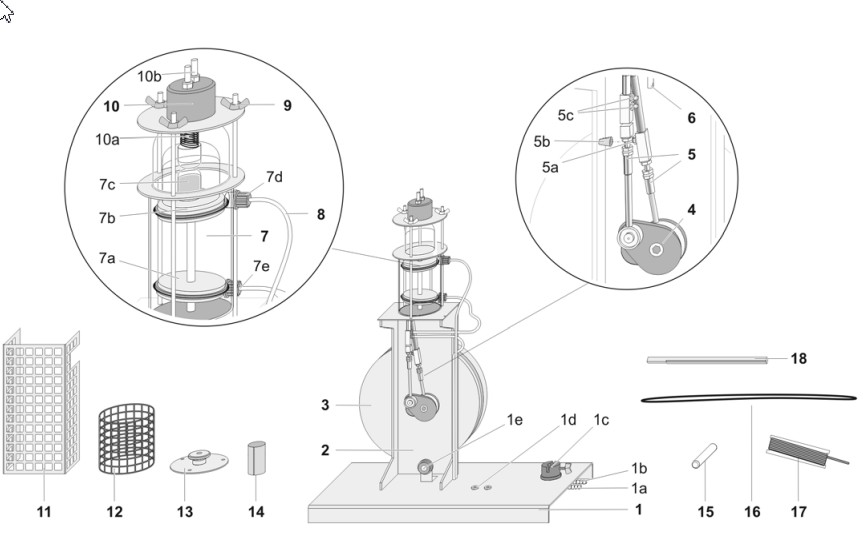
\includegraphics[scale=0.6]{Stirlingmotor}\caption{Aufbau des Stirlingmotors; 7a ist z.B. der Arbeitskolben und 7b der Verdrängungskolben;7d Kühlwasserabfluss;7e Kühlwasserzufluss;10a Heizspirale; entnommen aus dem Handbuch des Herstellers}\end{figure}

Wir betrieben den Stirlingmotor im Umlaufsinn 1. Als Wärmebäder benutzen wir zum Einen das Kühlwasser, was unser Wärmebad 2 darstellt, und das mit einer gewissen Geschwindigkeit $\text{d}m/\text{d}t$ durch das System gepumpt wurde, und zum Anderen eine Heizspirale im Zylinderkopf als Wärmebad 1. Dies ist so zu verstehen, dass wir hier durch die Heizwendel mit einer bestimmten elektrischen Leistung geheizt hatten, und abwarteten, bis sich die Temperatur im Zylinderkopf auf einen Gleichgewichtswert eingestellt hatte. In diesem Zustand können wir davon ausgehen das in guter Näherung die gesamte elektrische Leistung, in den thermodynamischen Prozess einfließt. Somit beträgt die vom Wärmebad 1 abgegebene Arbeit $\Delta{Q_{B_1}}=-P_{el}\cdot{\tau}$, wobei $\tau$ die Zeit eines Durchlaufs des Stirlingprozesses ist.
Die Wärme die das Wärmebad 2, also das Wasser aufnahm, bestimmten wir dadurch, dass wir die Temperatur $T_1$ des Kühlwassers unmittelbar nach Druchlauf durch den Stirlingmotor maßen. Aus der Differenz zur Temperatur des Kühltanks konnte die ans Wasser abgegebene Wärme berechnet werden.
\begin{equation*}\Delta{Q_{B_2}}=c_{V,\text{Wasser}}\,\Delta{T}\,\frac{\text{d}m}{\text{d}t}\,\tau\end{equation*}

Vor der eigentlichen Messung bestimmten wir noch die Reibungswärme $\Delta{Q_R}$, indem wir den Stirlingmotor bei geöffneten Zylinder betrieben. Dadurch traten keine Volumen und Druckänderungen auf und es fand kein thermodynamischer Prozess statt. Die Wärme, die dabei an das Wasser abgegeben wurde, entsprach hier $\Delta{Q_R}$.

Beim eigentlichen Versuch gingen wir dann wie oben beschrieben vor. Für 5 verschiedene Heizströme, warteten wir bis die Gleichgewichtstemperatur, die zwischen 10°C und 50°C lag, erreicht wurde, und maßen die Temperatur des Kühlwassers $T_1$.

Als zweiter Versuch betrieben wir den Stirlingmotor ohne externen Motor als Wärme-Kraft-Maschine. Dazu heizten wir den Motor über die Heizwendel im Zylinderkopf. Hierbei zeichnete ein Laser der auf ein Spiegelsystem im Stirlingmotor gerichtet war ein maßstabsgetreues p-V Diagramm an die Wand, das wir abzeichneten.

\section{Auswertung}
Wir betrieben den Stirlingmotor mit einer Frequenz von 5 Hz. Als erste Messung bestimmten wir die Durchflussmenge des Kühlwassers 5 mal.
\begin{table}[H]\centering\begin{tabular}{cc}gestoppte Zeit in s&gemessener Wasserdurchfluss in kg\\30&0.11\\60&0.19\\60&0.19\\120&0.36\\60&0.185\end{tabular}\caption{gemessener Wasserdurchfluss in Abhängigkeit der Zeitdauer}\end{table}

Daraus berechnet sich der Durchflussstrom zu 
$$\frac{\text{d}m}{\text{d}t}=3.22\,\frac{g}{s}$$
Die Temperatur des Wassertanks betrug $T_0=24.1°C$ und die Temperatur des Kühlwasser nach Durchlauf war im Leerlaufbetrieb $T_1=25.2°C$. Damit berechnet sich die Reibungswärme zu 
\begin{equation*}\Delta{Q_R}=2.958\,J\end{equation*}
Wir benutzten hierfür eine spezifische Wärmekapazität für Wasser von $C_{V,\text{Wasser}}=4.84\,kJ/(kg\,K)$ (Wikipedia).\newline\newline
Als nächstes maßen wir die Wärmemengen $\Delta{Q_{B_1}}$ und $\Delta{Q_{B_2}}$ für verschiedene Gleichgewichtstemperaturen $T_\text{zyl}$ im Zylinderkopf. Beziehungsweise wir maßen $T_1$, Heizstrom $I_H$, Heizspannung $U_H$ der Heizwendel, sowie die elektrische Leistung des externen Motors $P_M$.
\begin{table}[H]\centering\begin{tabular}{c|ccccc}
$T_\text{zyl}$ in °C&10&17.5&27&41.5&55\\\hline
$T_1$ in °C&28	&28.2	&28.4	&28.8	&29.3\\
$I_H$ in A&1.46	&1.57	&1.75	&1.93	&2.16\\
$U_H$ in V&13	&14	&15.4	&17	&19\\
$P_M$ in W&89	&87.6	&87.3	&85.4	&83.4\end{tabular}
\caption{Messung zur Bestimmung von $\Delta{Q_{B_1}}$ und $\Delta{Q_{B_2}}$ für verschieden Gleichgewichtstemperaturen. Die Temperatur des Kühlwassertanks $T_0$ ist unverändert 24.1°C}\end{table}
Daraus lassen sich die Wärmemengen berechnen. In Fortsetzung der Schreibweise aus der Theorie ist
\begin{align*}
\Delta{Q_{B_1}}=-\frac{P_H}{5\,Hz}\\
\Delta{Q_{B_2}}=C_V\,(T_1-T_0)\,\frac{\text{d}m}{\text{d}t}\,\frac{1}{5\,Hz}\end{align*}
\begin{table}[H]\centering\begin{tabular}{c|ccccc}
$T_\text{zyl}$ in °C&10&17.5&27&41.5&55\\\hline
$\Delta{Q_{B_1}}$ in J&-3.7966&-4.396&-5.39&-6.562&-8.208\\
$\Delta{Q_{B_2}}$ in J&10.488&11.025&11.563&12.639&13.983\end{tabular}
\caption{berechnete Wärmemengen}\end{table}
Hieraus lassen sich nach 
\begin{align*}W_{pV}=-(\Delta{Q_{B_1}}+\Delta{Q_{B_2}})+2\,\Delta{Q_R}\end{align*}
wiederum die jeweilige thermodynamisch genutzte Arbeit bestimmen
\begin{table}[H]\centering\begin{tabular}{c|ccccc}
$T_\text{zyl}$ in °C&10&17.5&27&41.5&55\\\hline
$W_{pV}$ in J&-0.776&-0.713&-0.257&-0.161&0.141\end{tabular}
\caption{thermodynamisch genutzte Arbeit}\end{table}
Hier sind natürliche einige Anmerkungen zumachen. Nach der Vorzeichenwahl in unserem Theorie Teil wird die thermodynamisch geleistete Arbeit negativ sobald die Temperatur im Zylinderkopf geringer ist als die des Kühlwassers. Dies gilt für die die Messung bei 41.5 °C nicht. Hier gibt es offensichtlich einen Fehler. Das erkläre ich damit, dass die Annahme, dass die gesamten Reibungsverluste durch $2\,\Delta{Q}_R$ ausgedrückt werden können, nicht zutrifft. \newline
Die Reibungswärme, die an den Zylinderkopf abgegeben wird, könnte größer sein, wodurch das zweifelhafte Messergebnis korrigiert werden könnte. Die fragliche Reibungswärme kann jedoch nicht seriös abgeschätzt werden. Es zweigt sich aber immerhin ein aus der Theorie erwarteter Übergang zwischen negativer und positiver thermodynamischer Arbeit. Dieser ist jedoch verschoben, was ich durch die Ungenauigkeit in der Reibungsmessung erkläre. Wenn wir nun die Messergebnisse so akzeptieren, können wir die daraus resultierenden Leistungszahlen bestimmen.\newline\newline
Die effektive äußere Kennzahl der Wärme Pumpe
\begin{equation*}\varepsilon_{A}=\frac{P_{el}\,\tau}{P_M\,\tau}\end{equation*}
sowie die innere Kennzahl
\begin{equation*}\varepsilon_{I}=\frac{P_{el}\,\tau}{W_{pV}}\end{equation*}
und den mechanischen Wirkungsgrad des externen Motors
\begin{align*}\eta=\frac{W_\text{Mech}}{P_M\,\tau}\\
=&\frac{-(-P_{el}\,\tau+\Delta{Q_{B_2}})+4\,\Delta{Q_R}}{P_M\,\tau}\end{align*}
sind in folgender Tabelle zusammengefasst
\begin{table}[H]\centering\begin{tabular}{c|ccccc}
$T_\text{zyl}$ in °C&10&17.5&27&41.5&55\\\hline
$\varepsilon_A$&0.21326	&0.25091	&0.30871	&0.38419	&0.49209\\
$\varepsilon_I$&-4.895&-6.162&-20.958&-40.8&58.378\\
$\eta$&0.289&0.297&0.324&0.337&0.363\end{tabular}
\caption{Leistungszahlen und Wirkungsgrad des Motors für die verschiedenen Temperaturen.}\end{table}

Bestimmen wir nun die Kennzahlen für das Wärmebad 2 (Wasser), betrachten wir den Aspekt der Wärmepumpe. Die äußere Kennzahl soll analog berechnet werden
\begin{equation*}\varepsilon_{A,W}=\frac{\Delta{Q_{B_2}}}{P_M\,\tau}\end{equation*}
Bei der Bestimmung der inneren Leistungszahl soll noch die Reibungswärme von$\Delta{Q_{B_2}}$ abgezogen werden.
\begin{equation*}\varepsilon_{I,W}=\frac{\Delta{Q_{B_2}}-\Delta{Q_R}}{P_M\,\tau}\end{equation*}
\begin{table}[H]\centering\begin{tabular}{c|ccccc}
$T_\text{zyl}$ in °C&10&17.5&27&41.5&55\\\hline
$\varepsilon_{A,W}$&0.589	&0.629	&0.662	&0.74	&0.838\\
$\varepsilon_{I,W}$&-9.709	&-11.309	&-33.46	&-60.192	&78.417\end{tabular}
\caption{äußere und innere Leistungszahl für die Wärmepumpe}\end{table}
Vor allem die innere Leistungszahl ist wieder mit sehr großer Unsicherheit verbunden, da ihre Größe stark von dem geringen Wert von $W_{ph}$ abhängt, der hier ja eine sehr große Unsicherheit hat.
Durch Interpolation der soliden äußeren Leistungszahl lässt sich die minimale Temperatur abschätzen.
\begin{figure}[H]\centering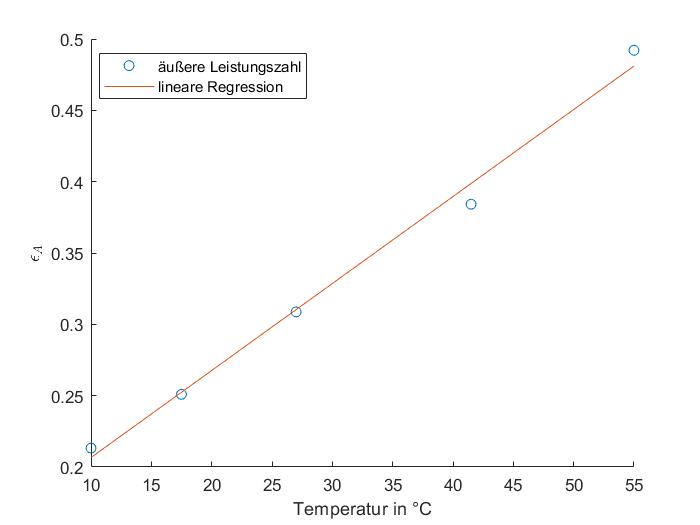
\includegraphics[scale=0.6]{Tempappro}\caption{lineare Regression an den Temperaturverlauf der äußeren Leistungszahl}\end{figure}
Die Approximation erfolgte durch die Funktion $\varepsilon_A(T)=0.0061\,T/K+0.1457$. Bei konstanter Motorleistung ist die minimal erreichte Temperatur durch den Fall gegeben, bei dem nicht zusätzlich durch die Heizspule geheizt wird und somit $\varepsilon_A=0$ gilt. Dies ist bei der Annahme eines linearen Verlauf bei -23.89°C gegeben.\newline\newline
Im zweiten Teil des Versuchs betrieben wir den Stirlingmotor als Wärme-Kraft-Maschine über eine Heizwedel im Zylinderkopf, die wir mit der konstanten Spannung und dem konstanten Strom $U_H=12.46\,V$; $I_H=1.29\,A$ betrieben. Es stellte sich eine Frequenz von 4 Hz ein, mit welcher der Kreisprozess durchlaufen wurde. Zur Messung der genutzten Arbeit, maßen wir den Verlauf von Druck und Volumen im Zylinder. Dazu wurden diese Größen auf Kippbewegungen eines Spiegels überführt, auf den ein Laser gerichtet wurde. Über Projektion auf ein Blatt Papier konnten wir so das pV Diagramm abzeichnen.
\begin{figure}[H]\centering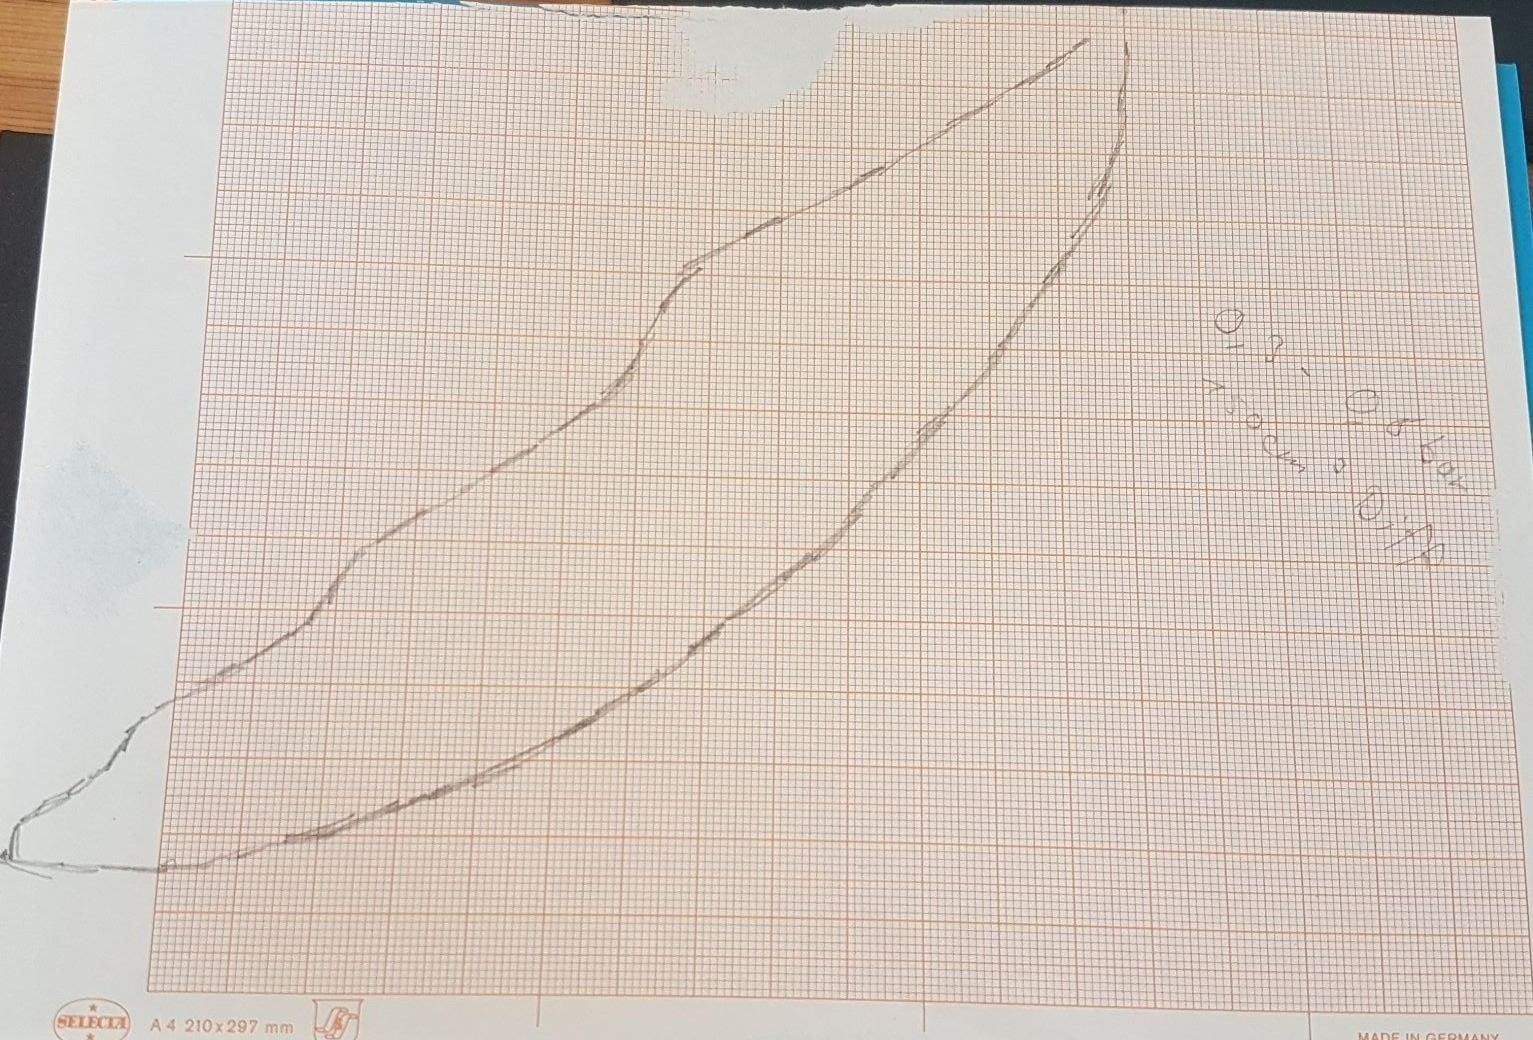
\includegraphics[scale=0.5]{pv diagramm2}\caption{abgezeichnetes pV Diagramm; die horizontale Ausdehnung beträgt \newline
150 $cm^3$ die vertikale beträgt 0.3 bar}\end{figure}
Das Volumen bewegt sich hierbei in einem Intervall von 150 $cm^3$ Differenz und der Druck zwischen 0.3 und 0.6 bar. Damit lies sich die genutzte Arbeit auf  $W=1.367\,J$ messen. Außerdem konnte die zur Berechnung des idealen stirlingschen Wirkungsgrads wichtige Größe $\Delta{Q}_1$ bestimmen. Vergleiche hierzu gegebenenfalls den Beginn des Theorie Teils. Wir maßen $\Delta{Q}_1=20.492\,J$. Es lässt sich nun der äußere elektrische Wirkungsgrad berechnen
$$\eta_{el}=\frac{W}{P_{el}}\cdot4\,Hz=0.3402$$
Dem geheizten Wärmereservoir wird immer eine Wärmemenge $-\Delta{Q}_{12}-\Delta{Q}_{23}$ abgeführt und ein Reibungsterm $\Delta{Q}_R$ zurückgeführt. Effektiv wird dem Reservoir also nur die Wärmemenge $\Delta{Q}_{B_1}=-\Delta{Q}_{12}-\Delta{Q}_{23}+\Delta{Q}_R$ abgeführt. Die Wärme die am thermodynamischen Prozess teilnimmt, ist daher größer als die dem Reservoir entzogenen Energie.
$$\Delta{Q}_{td}=\frac{P_{el}}{4\,Hz}+\Delta{Q}_{R,w}=W+(\Delta{Q}_{B_2}-\Delta{Q}_{R,zyl})$$
Diese Gleichung kann nach dem Reibungsterm im Zylinder umgestellt werden, wodurch dieser nochmal separat für diesen Versuch bestimmt werden kann. Wir bestimmten die an das Wärmebad 2 pro Umlauf abgegebene Wärme über den Temperaturunterschied zwischen Wassertank $T_1=25.1\,°C$ und dem Wasser, das unmittelbar den Kühlprozess verließ, $T_2=30.2\,°C$ auf $\Delta{Q}_{B_2}=17.143\,J$.
\begin{align*}\Rightarrow\;\Delta{Q}_{R,zyl}=W-\frac{P_{el}}{4\,Hz}+\Delta{Q}_{B_2}-\Delta{Q}_{R,w}=11.534\,J\end{align*}
Damit bestimmt sich der thermodynamische Wirkungsgrad zu
$$\eta_{td}=\frac{W}{Q_{td}}=0.0879$$
Dieser Wirkungsgrad ist vergleichsweise gering. Zur Berechnung orientierte ich mich an dem in der Anleitung zur Verfügung gestellten Schaubild
\begin{figure}[H]\centering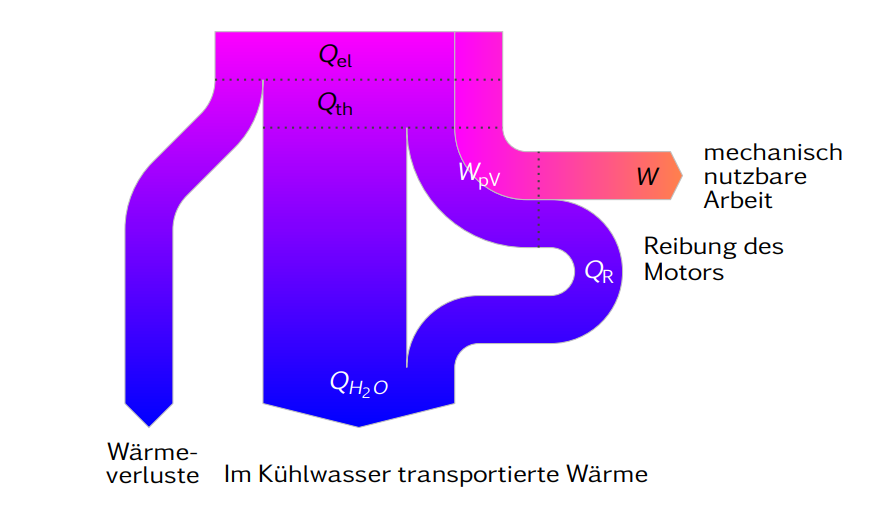
\includegraphics[scale=0.8]{Energiebilanz3}\caption{Energieflüsse beim Betrieb als Wärme-Kraft-Maschine; entnommen aus dem Anleitungsdokument}\end{figure}
Hier wird allerdings zur thermodynamisch genutzten Energie $\Delta{Q}_{td}$ noch der Term $C_V\,(T_1-T_3)$ hinzugezählt. Im idealen stirlingschen Wirkungsgrad wird dieser Term jedoch nicht berücksichtigt. Er ist nämlich definiert als
$$\eta_{id}=\frac{W}{\Delta{Q}_{12}}$$
Diese Größen wurden aus der Zeichnung bestimmt. Damit ist
$$\eta_{id}=0.667$$
Dieser Wirkungsgrad ist nochmal geringer als der thermodynamische, was natürlich nicht sein kann. Allerdings hat das abgezeichnete Bild auch nicht den typischen Verlauf des stirlingschen Kreisprozesses, es gibt keine Isochoren. Daher konnte $\Delta{Q}_{12}$ nicht genau bestimmt werden.

\section{Fazit}
Die Ergebnisse dieses Experiments sind teilweise mit sehr großer Unsicherheit zu verbunden. Sie widersprechen mit unter auf so starke Weise dem Experiment, dass man an der Korrektheit manches Zusammenhangs zweifeln muss. Allerdings sind diese Schwierigkeiten wohl auf große Fehlerquellen in der Konstruktion des Experiments zurückzuführen. Die schwerwiegendsten Fehlerquellen waren:
\begin{itemize}
\item{}die ungenaue Bestimmung, der im Prozess entstehenden Reibung
\item{}die wahre Heizmenge, die von der Heizspule dem System zugeführt wurde, ist nicht bekannt
\item{}die genaue Orientierung der pV Kurve ist möglicherweise nicht bekannt, was die Bestimmung der Wärmemenge $\Delta{Q}_{12}$ kompromittiert.
\item{}das aufgezeichnete pV Diagramm aus dem letzten Versuchsteil hatte ohne erkennbare Isochore nicht die typische Form des Stirling Kreisprozesses, was an der exakten Anwendbarkeit des verwendeten Modells zweifeln lässt
\end{itemize}
Aufgrund dieser Fehlerquellen und der nicht vollständig befriedigenden Übereinstimmung zwischen den erwarteten und gemessenen Werten lässt meine Beurteilung unseres Experiments als eher negativ ausfallen. Das grundlegende Konzept und Thema des Experiments und die theoretische Beschreibung dieses thermodynamischen Prozesses sind allerdings sehr interessant und machen den Versuch zu einer lohnenden Übung.


%\begin{note}An dieser Stelle möchte ich noch erwähnen, dass für den zweiten Umlaufsinn, die Reibungswärme, die sich im ersten Fall bei der Berechnung der mechanischen Arbeit der Motors aufsummiert, jetzt gerade aufhebt. Es gilt ohne Reibung
%\begin{align*}W_\text{Mech}=\Delta{Q_{B_1}}+\Delta{Q_{B_2}}\end{align*}
%und mit Reibung
%\begin{align*}W_\text{Mech}=&\Delta{Q_{B_1}}-\Delta{Q_R}+\Delta{Q_{B_2}}\Delta{Q_R}+2\,\Delta{Q_R}\\
%=&\Delta{Q_{B_1}}+\Delta{Q_{B_2}}\end{align*}\end{note}
















\end{document}